\section{Architettura CUDA}

CUDA è l'architettura di elaborazione parallela progettata e sviluppata da
NVIDIA che sfrutta la potenza di calcolo delle GPU (Graphics Processing Units)
per aumentare le prestazioni di alcuni tipi di software.
L'elaborazione sta lentamente migrando verso il paradigma di
\textit{co-processing} su CPU e GPU il quale prevede che l'esecuzione della
gran parte del carico computazionale venga demandata alla GPU, e i risultati
presi nuovamente in carico dalla CPU.
\\
Questo nuovo tipo di architettura ha trovato immediato seguito nel settore
della ricerca scientifica, dato che ha contribuito in particolare alla nascita
e al miglioramento di software per la simulazione di fenomi fisici e
biologici.

\paragraph{Specifiche Hardware}\mbox{}
\\
Generalmente l'hardware può cambiare con l'avvento di
nuove generazioni di GPU ma la struttura generale si basa sempre sul concetto di
Streaming Multiprocessors (SMs) \cite{nickolls2010gpu}

\begin{figure}[H]
    \centering
    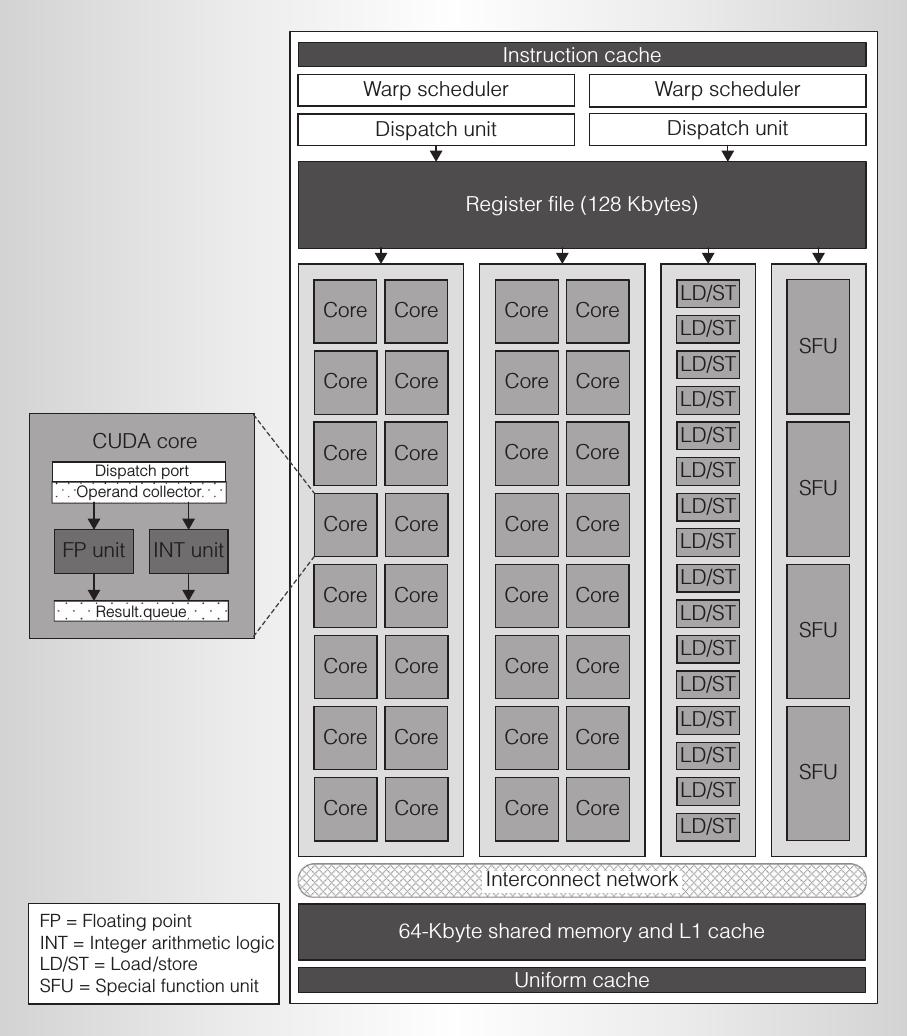
\includegraphics[scale=0.4]{fermi_sm}
    \caption{Streaming Multiprocessor dell'architettura Fermi 
        \cite{nickolls2010gpu}}
\end{figure}

\paragraph{Astrazione Software}\mbox{}
\\
Dato che vengono periodicamente rilasciate nuove versione dell'architettura
hardware delle schede, NVIDIA ha sviluppato delle API per dialogare con la GPU
che sono indipendenti dall'architettura del device utilizzato, rendendo
così possibile lo sviluppo di software portabile su molte schede che
supportano CUDA.
\\
Il modello astratto definisce tre tipologie di oggetti:

\begin{itemize}
    \item
        Thread: singole unità di calcolo, eseguono il codice sorgente;
    \item
        Thread Block: insieme logico di Thread.
        I Thread appartenenti
        allo stesso Thread Block hanno accesso ad un'area di memoria
        condivisa e accessibile solamente da questi ultimi
        (oltre alla memoria globale della GPU);
        È inoltre possibile ottenere la sincronizzazione di tutti i
        Thread appartenenti al medesimo Thread Block;
    \item
        Grid: insieme logico di Thread Block. Non è stata
        prevista un'area di memoria condivisa da tutta la Grid
        e fino ad ora non esiste una primitiva per la sincronizzazione fra
        Thread Block di una specifica Grid, ed è quindi
        obbligatorio procedere alla sincronizzazione di tutti i Thread
        mediante la funzione \textit{cudaDeviceSynchronize()}.
\end{itemize}

\begin{figure}[H]
    \centering
    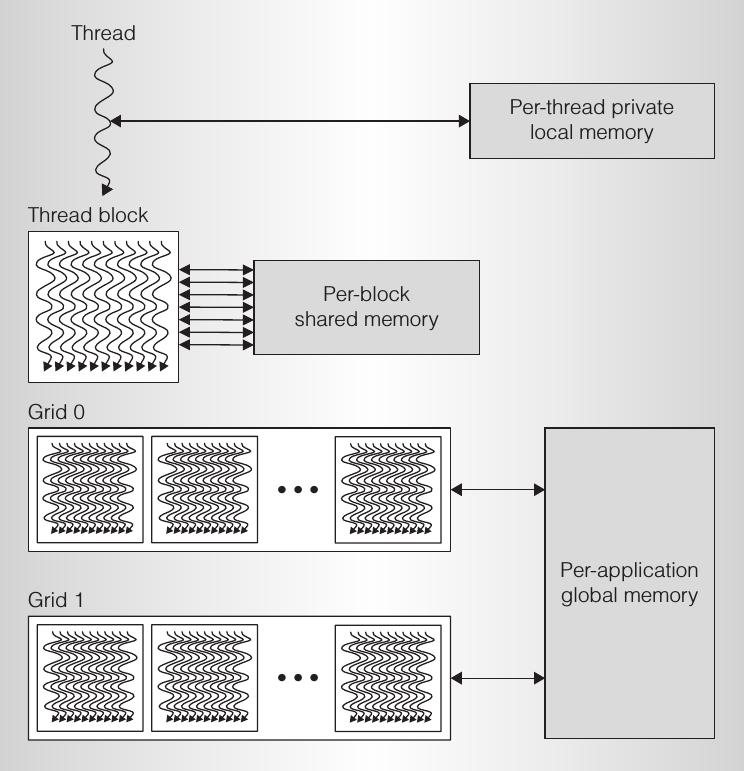
\includegraphics[scale=0.5]{cuda_astraction}
    \caption{Schema della gerarchia di Thread, Thread block, e
        \textit{Grid} \cite[p.~59]{nickolls2010gpu}}
\end{figure}

Le procedure che vengono eseguite sulla GPU vengono chiamate Kernel
(identificabili grazie al prefisso \textit{\_\_global\_\_})
ed è possibile specificarne la dimensione, ovvero decidere quanti
Thread, Thread block e Grid verranno assegnati
all'esecuzione del codice invocato.
\\
\lstinputlisting[label=kernel, language=C++,
    caption={Esempio di invocazione GPU kernel},
    style=custom]
    {Code/simple_kernel.c}

Come è possibile notare nell'esempio di codice \ref{kernel}, si sta invocando
l'esecuzione di un Kernel specificando l'utilizzo di 8 Thread Block e
32 Thread per blocco (quando non specificato, il numero delle
Grid da utilizzare ha come valore di default 1). In generale il numero totale di
Thread che verranno utilizzati per la computazione del Kernel è
$$\Gamma * B * T$$ dove $\Gamma, B, T$
sono rispettivamente
il numero di Grid, il numero di Thread Block e il numero
di Thread che si vuole utilizzare.

La possibilità di modificare la suddivisione del Kernel tra Grid e Thread Block
si rivela molto utile nell'elaborazione di strutture dati non
particolarmente complesse, come gli array.
Infatti è sufficiente invocare un Kernel con numero di Thread
uguale (o maggiore) al numero di elementi dell'array e assegnare la
computazione di ogni elemento ad un singolo e specifico Thread.
\\
Esiste però un limite al numero di Thread per Thread Block che è possibile
dichiarare (nelle nuove versioni di CUDA è 1024), dunque per ottenere
l'id globale del Thread relativo al Kernel eseguito bisogna avvalersi anche
del numero di Grid e Thread Block richiesti durante l'invocazione del Kernel,
secondo la seguente relazione:
$$\tau + (\beta * B) * (\gamma * G)$$
dove $\Gamma, B, T$ sono rispettivamente il numero di Grid,
il numero di Thread Block, e il numero di Thread che
devono essere utilizzati e $\gamma, \beta, \tau$ sono gli id locali
associati alle Grid, Thread Block e
Thread con $\gamma < \Gamma, \beta < B, \tau < T$.
\\
\lstinputlisting[label=threadid, language=C++,
    caption={Esempio di calcolo dell'id globale associato ad un Thread durante
            l'esecuzione di un Kernel},
    style=custom]
    {Code/thread_id.c}
